\begin{exercise}
      {ID-6b0510e2b36519987fed8db12a9cdc9c114d5a65}
      {Ablesen und rechnen}
  \ifproblem\problem\par
    % <PROBLEM>
    Gib die Funktionsgleichung der abgebildeten
    Parabel in Normalform an, und bestimme ihre
    Nullstellen exakt:
    \begin{center}
    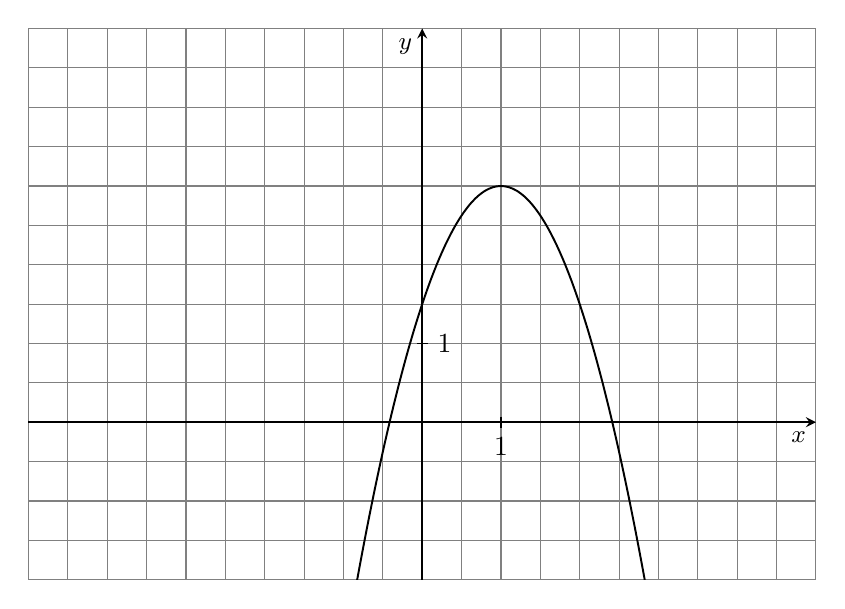
\begin{tikzpicture}[scale=1.000]
      % grid
      \draw[draw=black!50!white] (-5.000, -2.000) grid[step=0.5] (5.000, 5.000);
      % x-axis
      \draw[line width=0.6pt, ->, >=stealth] (-5.000, 0) -- (5.000, 0) node[below left] {\small$x$};
      % x scale
      \draw (1, 2pt) -- (1, -2pt) node[below] {1};
      % y-axis
      \draw[line width=0.6pt, ->, >=stealth] (0, -2.000) -- (0, 5.000) node[below left] {\small$y$};
      % y scale
      \draw (-2pt, 1) -- (2pt, 1) node[right] {1};
      % function: f(x)=-\num{1.5}x^{2}+\num{3}x+\num{1.5}
      \begin{scope}[line width=0.7pt]
        \clip (-5.000, -2.000) rectangle (5.000, 5.000);
        \draw plot[smooth] coordinates
        {
          ( -5.000,  -5.000) ( -4.900,  -5.000) ( -4.800,  -5.000)
          ( -4.700,  -5.000) ( -4.600,  -5.000) ( -4.500,  -5.000)
          ( -4.400,  -5.000) ( -4.300,  -5.000) ( -4.200,  -5.000)
          ( -4.100,  -5.000) ( -4.000,  -5.000) ( -3.900,  -5.000)
          ( -3.800,  -5.000) ( -3.700,  -5.000) ( -3.600,  -5.000)
          ( -3.500,  -5.000) ( -3.400,  -5.000) ( -3.300,  -5.000)
          ( -3.200,  -5.000) ( -3.100,  -5.000) ( -3.000,  -5.000)
          ( -2.900,  -5.000) ( -2.800,  -5.000) ( -2.700,  -5.000)
          ( -2.600,  -5.000) ( -2.500,  -5.000) ( -2.400,  -5.000)
          ( -2.300,  -5.000) ( -2.200,  -5.000) ( -2.100,  -5.000)
          ( -2.000,  -5.000) ( -1.900,  -5.000) ( -1.800,  -5.000)
          ( -1.700,  -5.000) ( -1.600,  -5.000) ( -1.500,  -5.000)
          ( -1.400,  -5.000) ( -1.300,  -4.935) ( -1.200,  -4.260)
          ( -1.100,  -3.615) ( -1.000,  -3.000) ( -0.900,  -2.415)
          ( -0.800,  -1.860) ( -0.700,  -1.335) ( -0.600,  -0.840)
          ( -0.500,  -0.375) ( -0.400,   0.060) ( -0.300,   0.465)
          ( -0.200,   0.840) ( -0.100,   1.185) (  0.000,   1.500)
          (  0.100,   1.785) (  0.200,   2.040) (  0.300,   2.265)
          (  0.400,   2.460) (  0.500,   2.625) (  0.600,   2.760)
          (  0.700,   2.865) (  0.800,   2.940) (  0.900,   2.985)
          (  1.000,   3.000) (  1.100,   2.985) (  1.200,   2.940)
          (  1.300,   2.865) (  1.400,   2.760) (  1.500,   2.625)
          (  1.600,   2.460) (  1.700,   2.265) (  1.800,   2.040)
          (  1.900,   1.785) (  2.000,   1.500) (  2.100,   1.185)
          (  2.200,   0.840) (  2.300,   0.465) (  2.400,   0.060)
          (  2.500,  -0.375) (  2.600,  -0.840) (  2.700,  -1.335)
          (  2.800,  -1.860) (  2.900,  -2.415) (  3.000,  -3.000)
          (  3.100,  -3.615) (  3.200,  -4.260) (  3.300,  -4.935)
          (  3.400,  -5.000) (  3.500,  -5.000) (  3.600,  -5.000)
          (  3.700,  -5.000) (  3.800,  -5.000) (  3.900,  -5.000)
          (  4.000,  -5.000) (  4.100,  -5.000) (  4.200,  -5.000)
          (  4.300,  -5.000) (  4.400,  -5.000) (  4.500,  -5.000)
          (  4.600,  -5.000) (  4.700,  -5.000) (  4.800,  -5.000)
          (  4.900,  -5.000) (  5.000,  -5.000)
        };
      \end{scope}
    \end{tikzpicture}
    \end{center}
    % </PROBLEM>
  \fi
  %\ifoutline\outline\par
    % <OUTLINE>
    % </OUTLINE>
  %\fi
  \ifoutcome\outcome\par
    % <OUTCOME>
    Da man die Koordinaten des Scheitelpunktes
    relativ gut ablesen kann, ist es einen Versuch
    wert, zunächst die Scheitelpunktform der
    Parabel zu bestimmen. Die Scheitelpunktform
    einer Parabel hat folgende Struktur:
    \begin{equation*}
      f(x)=a(x-d)^2+e
      \quad
      \text{mit dem Scheitelpunkt}
      \quad
      S\left(d\;\middle|\;e\right)
    \end{equation*}
    Für die abgebildete Parabel erhält man also
    folgendes Zwischenergebnis:
    \begin{equation*}
      f(x)=a(x-1)^2+3
    \end{equation*}
    Um den Skalierungsfaktor $a$ bestimmen zu
    können, benötigt man einen weiteren Punkt
    $P$ auf der Parabel, dessen Koordinaten
    man genau ablesen kann.
    Hier bietet sich zum Beispiel der
    $y$-Achsen\-ab\-schnitt
    $P\left(0\;\middle|\;\num{1.5}\right)$ an.
    Die Scheitelpunktform lässt sich dann nach
    $a$ auflösen, und der Parameter $a$
    kann mit den abgelesenen Werten berechnet
    werden:
    \begin{equation*}
      \begin{split}
        f(x)&=a(x-d)^2+e
        \quad\Rightarrow\quad
        \frac{f(x)-e}{(x-d)^2}=a
        \\
        a&=\frac{\num{1.5}-\num{3}}{(\num{0}-\num{1})^2}
        =\num{-1.5}
      \end{split}
    \end{equation*}
    Die Scheitelpunktform der abgebildeten Parabel
    lautet also:
    \begin{equation*}
      f(x)=\num{-1.5}\cdot(x-1)^2+3
    \end{equation*}
    Das Ausmultiplizieren der Scheitelpunktform
    liefert die gesuchte Normalform:
    \begin{equation*}
      \begin{split}
        f(x)&=\num{-1.5}\cdot(x-1)^2+3\\
            &=\num{-1.5}\cdot(x^2-2x+1)+3\\
            &=\num{-1.5}x^2+3x-\num{1.5}+3\\
            &=\num{-1.5}x^2+3x+\num{1.5}
      \end{split}
    \end{equation*}
    Sobald man die Normalform der Parabel kennt,
    kann man ihre Nullstelllen mit Hilfe der
    $pq$-Formel bestimmen:
    \begin{alignat*}{3}
      \relax&\quad
      &
      0&=\num{-1.5}x^2+3x+\num{1.5}
      &
      \quad&|:(\num{-1.5})
      \\
      \Leftrightarrow&\quad
      &
      0&=x^2-2x-1
      &
      \quad&|\;\text{$pq$-Formel}
      \\
      \Leftrightarrow&\quad
      &
      x_{1,2}&=-\frac{-2}{2}\pm\sqrt{\left(\frac{-2}{2}\right)^2-(-1)}
      &
      \quad&\relax
      \\
      \relax&\quad
      &
      &=1\pm\sqrt{2}
      &
      \quad&\relax
      \\
      \Leftrightarrow&\quad
      &
      x&=1-\sqrt{2}\quad\lor\quad
      x=1+\sqrt{2}
      &
      \quad&\relax
    \end{alignat*}
    % </OUTCOME>
  \fi
\end{exercise}
